\documentclass[a4paper]{article}
\usepackage{cmap}
\usepackage[utf8]{inputenc}
\usepackage[T2A]{fontenc}
\usepackage[english,russian]{babel} 
\usepackage[left=15mm, top=15mm, right=15mm, bottom=42mm, nohead, nofoot]{geometry}
\usepackage{blindtext}  % рыба-текст
\usepackage{graphicx}  % изобржаения
\usepackage{float} % плавающие объекты
\usepackage{wrapfig}  % изобржаения
\usepackage{tikz} % графика
\usepackage{mdframed} % рамки
\usepackage{xcolor} % определение цветов
\usepackage{nicefrac} % красивые дроби
\usepackage{cancel} % сокращение
\usepackage{amsmath,amsfonts,amssymb} % математический пакет
\usepackage{hyperref}  % гиперссылки
\usepackage{fancybox,fancyhdr} % хедер и футер
\usepackage{listings} % код
\usepackage[skip=5pt]{caption} % расстояние между подписью и картинкой
\pagestyle{fancy}
\fancyhf{}
\fancyhead[L]{Лабораторная работа №4}
\fancyhead[R]{\textit{Линейная фильтрация}}
\fancyfoot[C]{\thepage}
\headsep=8mm    
\footskip=20mm
\setlength{\parindent}{0em}
\setlength{\parsep}{0em}

\definecolor{urlcolor}{HTML}{3454D1}
\definecolor{linkcolor}{HTML}{3454D1}
\hypersetup{pdfstartview=FitH, linkcolor=linkcolor, urlcolor=urlcolor, colorlinks=true}

\definecolor{strings}{rgb}{0,0.6,0}
\definecolor{comments}{rgb}{0,0.3,0}
\definecolor{numbers}{rgb}{0.5,0.5,0.5}
\definecolor{keywords}{rgb}{0.09,0.61,0.95}
\definecolor{background}{rgb}{0.97,0.97,0.97}
\lstdefinestyle{codestyle}{
    backgroundcolor=\color{background},
    commentstyle=\color{comments},
    keywordstyle=\color{keywords},
    stringstyle=\color{strings},
    numberstyle=\tiny\color{numbers},
    basicstyle=\ttfamily\footnotesize,
    breakatwhitespace=false,
    breaklines=true,
    captionpos=b,
    inputencoding=utf8,
    keepspaces=true,
    numbers=left,
    numbersep=5pt,
    showspaces=false,
    showstringspaces=false,
    showtabs=false,
    tabsize=2,
    extendedchars=true,
    literate=
    {а}{{\cyra}}1
    {б}{{\cyrb}}1
    {в}{{\cyrv}}1
    {г}{{\cyrg}}1
    {д}{{\cyrd}}1
    {е}{{\cyre}}1
    {ж}{{\cyrzh}}1
    {з}{{\cyrz}}1
    {и}{{\cyri}}1
    {й}{{\cyrishrt}}1
    {к}{{\cyrk}}1
    {л}{{\cyrl}}1
    {м}{{\cyrm}}1
    {н}{{\cyrn}}1
    {о}{{\cyro}}1
    {п}{{\cyrp}}1
    {р}{{\cyrr}}1
    {с}{{\cyrs}}1
    {т}{{\cyrt}}1
    {у}{{\cyru}}1
    {ф}{{\cyrf}}1
    {х}{{\cyrh}}1
    {ц}{{\cyrc}}1
    {ч}{{\cyrch}}1
    {ш}{{\cyrsh}}1
    {щ}{{\cyrshch}}1
    {ъ}{{\cyrhrdsn}}1
    {ы}{{\cyrery}}1
    {ь}{{\cyrsftsn}}1
    {э}{{\cyrerev}}1
    {ю}{{\cyryu}}1
    {я}{{\cyrya}}1
    {А}{{\CYRA}}1
    {Б}{{\CYRB}}1
    {В}{{\CYRV}}1
    {Г}{{\CYRG}}1
    {Д}{{\CYR96}}1
    {Е}{{\CYRE}}1
    {Ж}{{\CYRZH}}1
    {З}{{\CYRZ}}1
    {И}{{\CYRI}}1
    {Й}{{\CYRISHRT}}1
    {К}{{\CYRK}}1
    {Л}{{\CYRL}}1
    {М}{{\CYRM}}1
    {Н}{{\CYRN}}1
    {О}{{\CYRO}}1
    {П}{{\CYRP}}1
    {Р}{{\CYRR}}1
    {С}{{\CYRS}}1
    {Т}{{\CYRT}}1
    {У}{{\CYRU}}1
    {Ф}{{\CYRF}}1
    {Х}{{\CYRH}}1
    {Ц}{{\CYRC}}1
    {Ч}{{\CYRCH}}1
    {Ш}{{\CYRSH}}1
    {Щ}{{\CYRSHCH}}1
    {Ъ}{{\CYRHRDSN}}1
    {Ы}{{\CYRERY}}1
    {Ь}{{\CYRSFTSN}}1
    {Э}{{\CYREREV}}1
    {Ю}{{\CYRYU}}1
    {Я}{{\CYRYA}}1
}

\lstset{style=codestyle}

\addto\captionsrussian{
  \renewcommand{\contentsname}
    {\centering Содержание}
}
\newcommand{\addsection}[1]{
    \phantomsection
    \addcontentsline{toc}{section}{#1}
    \section*{\centering #1}
}
\newcommand{\addsubsection}[1]{
    \phantomsection
    \addcontentsline{toc}{subsection}{#1}
    \subsection*{\centering #1}
}
\newcommand{\addsubsubsection}[1]{
    \phantomsection
    \addcontentsline{toc}{subsubsection}{#1}
    \subsubsection*{\centering #1}
}

\newmdenv[
  leftmargin = 0.5em,
  skipabove = 0.5em,
  skipbelow = 0.5em,
  linewidth = 1pt,
  rightline = false,
  topline = false,
  bottomline = false
]{quotebox}

\newlength{\tempheight}
\newcommand{\Let}{
\mathbin{\text{\settoheight{\tempheight}{\mathstrut}\raisebox{0.4\pgflinewidth}{
\tikz[baseline=0.5ex,line cap=round,line join=round] \draw (0,0) --++ (0.3em,0) --++ (0,2.3ex) --++ (-0.3em,0);
}}}}
\newcommand*\squared[1]{\tikz[baseline=(char.base)]{
            \node[shape=rectangle,draw,inner sep=4pt] (char) {#1};}}
\newcommand*\msquared[1]{\tikz[baseline=(char.base)]{
            \node[shape=rectangle,draw,inner sep=4pt] (char) {$\displaystyle #1$};}}
\newcommand{\at}{\biggr\rvert}
\newcommand{\shiftright}[3]{\makebox[#2][r]{\makebox[#1][l]{#3}}}
\newcommand{\e}{\;\text{e}}
\let\oldint\int
\def\int{\oldint\limits}
\DeclareRobustCommand{\divby}{%
  \mathrel{\vbox{\baselineskip.65ex\lineskiplimit0pt\hbox{.}\hbox{.}\hbox{.}}}%
}

\newcommand\NB{\textbf{N\kern-0.32em\textcolor{red}{B}}}

\begin{document}
\begin{titlepage}
    \begin{center}
        Федеральное государственное автономное образовательное \\ учреждение высшего образования \\[6pt]
        САНКТ-ПЕТЕРБУРГСКИЙ НАЦИОНАЛЬНЫЙ \\ ИССЛЕДОВАТЕЛЬСКИЙ УНИВЕРСИТЕТ ИТМО \\[16pt]
        Факультет систем управления и робототехники \\[26em]
        Лабораторная работа №4 \\[0.5em]
        \textbf{\MakeUppercase{Линейная фильтрация}}
    \end{center}\vspace{12em}
    \begin{flushright}
        Студент: Овчинников П.А.\\
        Поток: ЧАСТ.МЕТ. 1.3 \\[0.5em]
        Преподаватель: Перегудин А.А. \\
        Пашенко А.В.
    \end{flushright}\vspace{8em}
    \begin{center}
        {\small Санкт-Петербург \\ 2024}
    \end{center}
\end{titlepage}
\setcounter{page}{2}
\tableofcontents\newpage

% MARK: спектральное дифференцирование
\addsection{Спектральное дифференцирование}
Зададим $t \in [-25, 25]$ и рассмотрим сигнал $y(t)$, представляющий из себя зашумлённую синусоиду:
$$y(t) = \sin(t)+0.1\left(\text{rand}\left(\text{size}(t)\right)-0.5\right)$$\vspace{-2em}
\begin{figure}[H]
    \centering 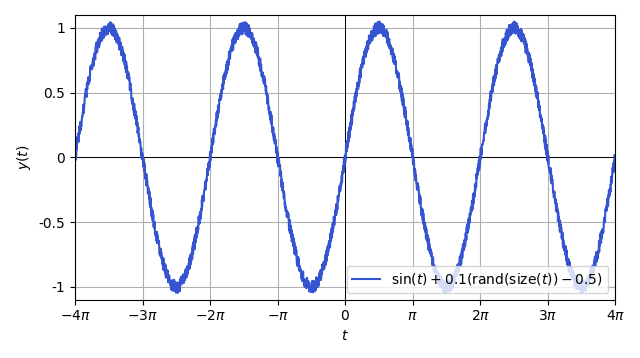
\includegraphics[width=0.66\textwidth]{sources/first/1_signal.png}
    \caption{Сигнал $y(t)$}
\end{figure}
Теперь найдём численную производную этого сигнала с помощью формулы поэлементного дифференцирования:
$$y'(t) = \frac{y(t+1)-y(t)}{dt},\qquad dt\text{ --- шаг дискретизации}$$\vspace{-2em}
\begin{figure}[H]
    \centering 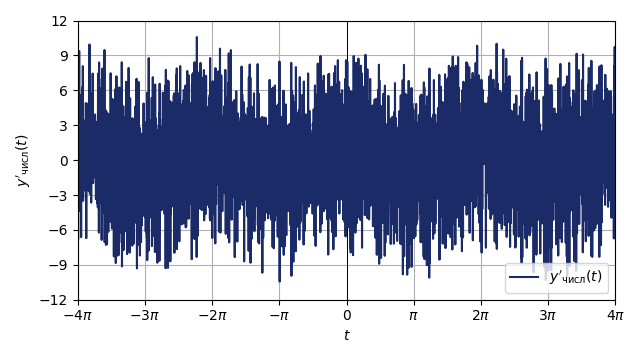
\includegraphics[width=0.66\textwidth]{sources/first/2_numerical_diff.png}
    \caption{Численная производная сигнала}
\end{figure}
Как мы видим, численная производная сигнала имеет колосальное количества шума. Это связано с резкими скачками функции на каждом шаге дискретизации, вызванными шумом. Конечно, здесь заметна истинная производная сигнала $\cos(t)$, но всё же шум вносит свои неисправимые коррективы.\\[0.5em]
Теперь найдём спектральную производную сигнала. Для этого применим преобразование Фурье к сигналу $y(t)$, а затем умножим полученный Фурье-образ на $i\omega$. После этого применим обратное преобразование Фурье к полученному произведению --- и так мы получим спектральную производную сигнала.\\[0.5em]
Такая манипуляция основана на свойстве Фурье-образа: $\mathcal{F}\left\{ \frac{d}{dt} f \right\} = 2\pi iv\mathcal{F}\left\{ f \right\}$. В зависимости от того, каким преобразованием мы пользуемся, унитарным или неунитарным, нам может потребоваться дополнительный множитель $2\pi$. В этой работе мы пользуемся унитарным преобразованием к угловой частоте, поэтому $i\omega$ достаточно.\\[0.5em]
Для начала рассмотрим Фурье-образ сигнала и его преобразование после умножения на $i\omega$:
\begin{figure}[H]
    \begin{minipage}{0.49\textwidth}
        \centering 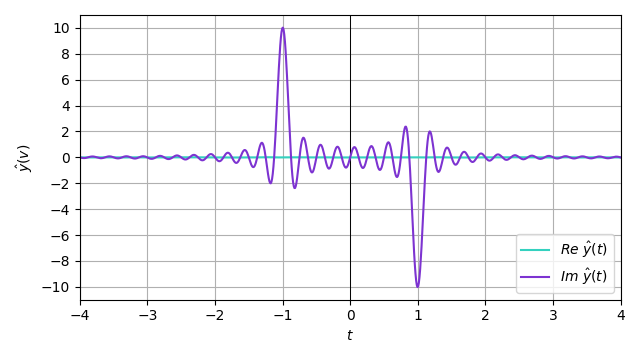
\includegraphics[width=\textwidth]{sources/first/3_fft.png}
        \caption{Фурье-образ сигнала}
    \end{minipage}\hfill
    \begin{minipage}{0.49\textwidth}
        \centering 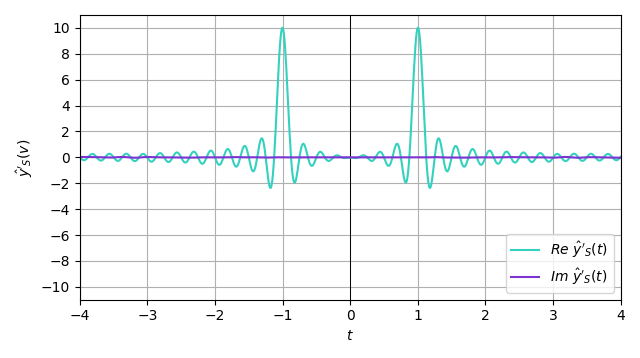
\includegraphics[width=\textwidth]{sources/first/4_spectral_fft.png}
        \caption{Фурье-образ после умножения на $i\omega$}
    \end{minipage}
\end{figure}
Как мы видим, весь образ оказался в мнимой части. Теперь применим обратное преобразование к получившемуся образу --- получим спектральную производную. Так она выглядит в сравнении с истинной производной $\cos(t)$:
\begin{figure}[H]
    \centering 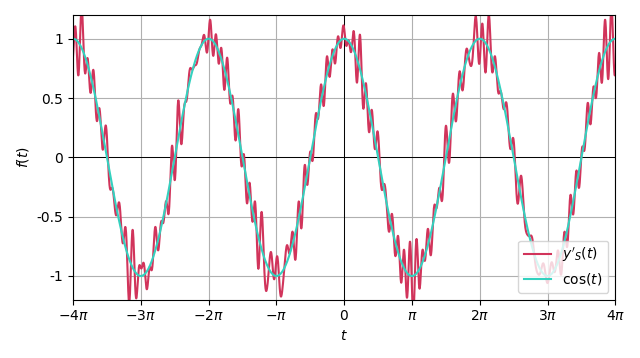
\includegraphics[width=0.66\textwidth]{sources/first/5_diff_cmp.png}
    \caption{Сравнение спектральной производной и истинной производной сигнала}
\end{figure}
Как мы видим, спектральная производная сигнала практически совпадает с истинной производной сигнала, в то время как численная производная сигнала содержит колоссальное количество шума. Поэтому спектральную производную можно рассматривать как способ найти приблежённую производную сигнала даже с наличием шумов в нём.\\[0.5em]
\NB: Здесь стоит отметить недостаток спектрального дифференцирования. Мы рассматривали промежуток $[-25, 25]$, достаточный для того, чтобы спектральное дифференцирование работало хорошо. Но если мы рассмотрим больший промежуток, например, как в условии задания, $[-100, 100]$, то Фурье-образ будет принимать на себя всё больше и больше шума, что приведёт к ухудшению качества спектральной производной:
\begin{figure}[H]
    \begin{minipage}{0.33\textwidth}
        \centering 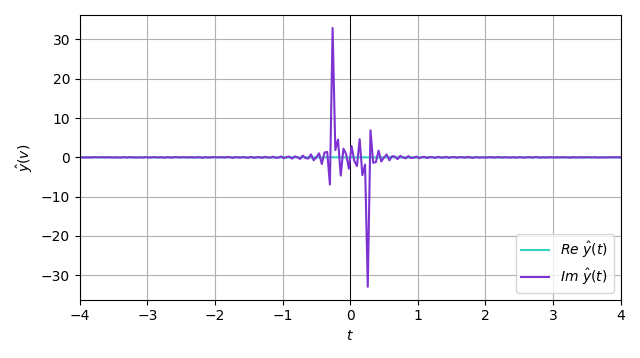
\includegraphics[width=\textwidth]{sources/first/6_wider_fft.png}
        \caption{Фурье-образ сигнала}
    \end{minipage}\hfill
    \begin{minipage}{0.33\textwidth}
        \centering 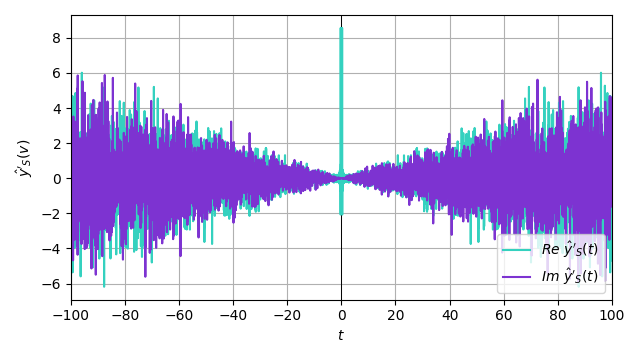
\includegraphics[width=\textwidth]{sources/first/7_wider_spectral_fft.png}
        \caption{Фурье-образ $\cdot\ i\omega$}
    \end{minipage}\hfill
    \begin{minipage}{0.33\textwidth}
        \centering 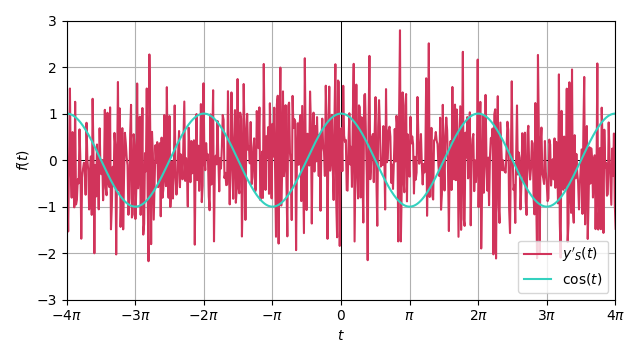
\includegraphics[width=\textwidth]{sources/first/8_wider_diff_cmp.png}
        \caption{Сравнение производных}
    \end{minipage}
\end{figure}

% MARK: линейные фильтры
\addsection{Линейные фильтры}
Рассмотрим сигнал, представляющий собой зашумленную прямоугольную волну:
$$u(t) = g(t) + b\left( \text{rand}\left( \text{size}(t) \right) - 0.5 \right) + c\sin(d\cdot t)$$\vspace{-2.3em}
\addsubsection{Фильтр первого порядка}
Для выполнения задания с фильтром первого порядка нам понадобится только случайный шум в сигнале, поэтому $c = 0$. Необходимо пропустить сигнал $u$ через фильтр первого порядка, являющийся передаточной функцией:
$$W_1(p) = \frac{1}{Tp + 1}$$
И, изменяя постоянную времени $T$ и параметр $a$, исследовать их влияние на эффективность фильтрации.\\[0.5em]
Пусть $a = 5$ --- это амплитуда прямоугольной волны, $b = 1$ --- амплитуда шума, а касательно постоянной времени предположим $T = 0.5$. Пропустим сигнал с такими параметрами через такой фильтр и посмотрим на результат:
\begin{figure}[H]
    \centering 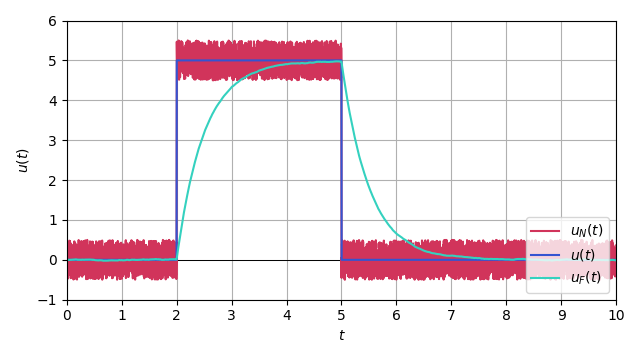
\includegraphics[width=0.66\textwidth]{sources/second/part1/a=5 T=0.5/1_signal_cmp.png}
    \caption{Графики исходного сигнала $u(t)$, зашумлённого сигнала $u_N(t)$ и отфильтрованного сигнала $u_F(t)$}
\end{figure}
Фронт и спад прямоугольной волны стали более плавными, а шум уменьшился. Это связано с тем, что фильтр уменьшает высокочастотные компоненты сигнала. Теперь посмотрим на модули Фурье-образов сигналов:
\begin{figure}[H]
    \centering 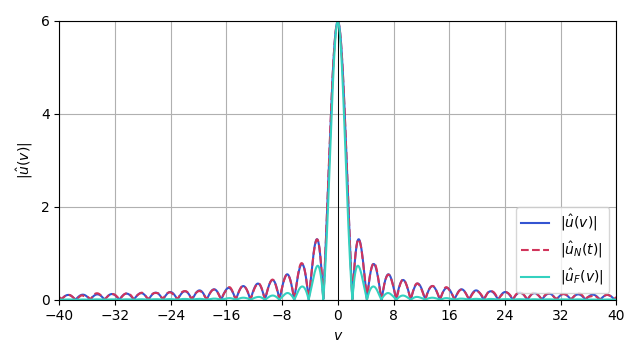
\includegraphics[width=0.66\textwidth]{sources/second/part1/a=5 T=0.5/2_fft_cmp.png}
    \caption{Графики модулей фурье-образов исходного, зашумлённого и отфильтрованного сигналов}
\end{figure}
По образу видно, что фильтр плавно уменьшает высокочастотные компоненты, что и привело к сглаживанию.\\[0.5em]
Посмотрим на АЧХ фильтра:
\begin{figure}[H]
    \centering 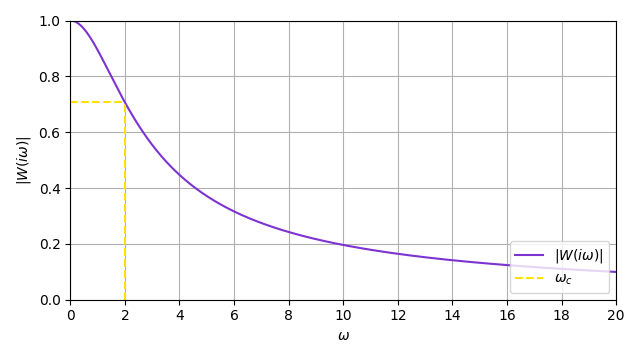
\includegraphics[width=0.66\textwidth]{sources/second/part1/a=5 T=0.5/3_filter.png}
    \caption{АЧХ фильтра первого порядка при $T = 0.5$}
\end{figure}
Здесь и в следующих графиках для наглядности отмечена частота среза $\omega_c$. Для этой частоты выполняется условие $|W_1(j\omega_c)| = \nicefrac{1}{\sqrt{2}}$. Для фильтра первого порядка эта частота среза равна $\omega_c = \nicefrac{1}{T} = \nicefrac{1}{0.5} = 2$.\\[0.5em]
Теперь попробуем уменьшить постоянную времени фильтра до $T = 0.1$:
\begin{figure}[H]
    \centering 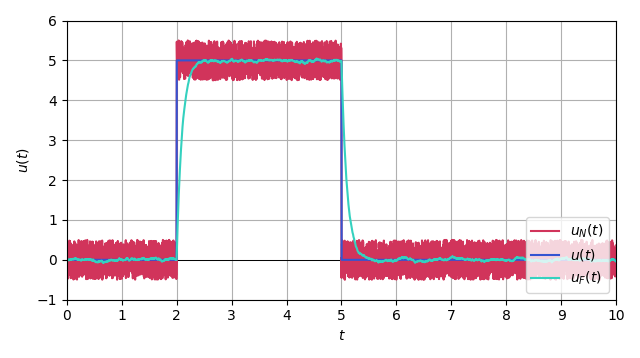
\includegraphics[width=0.66\textwidth]{sources/second/part1/a=5 T=0.1/1_signal_cmp.png}
    \caption{Графики исходного, зашумлённого и отфильтрованного сигналов при $T = 0.1$}
\end{figure}\vspace{-1em}
\begin{figure}[H]
    \begin{minipage}{0.49\textwidth}
        \centering 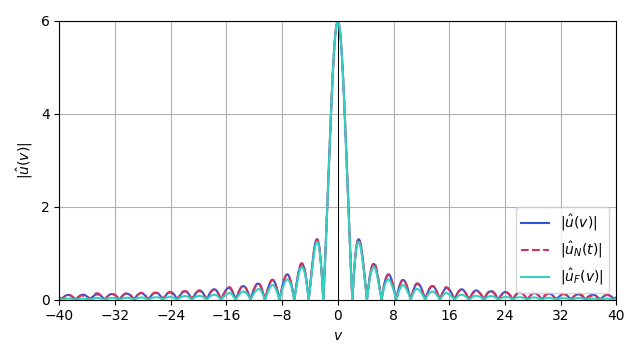
\includegraphics[width=\textwidth]{sources/second/part1/a=5 T=0.1/2_fft_cmp.png}
        \caption{Модули Фурье-образов сигналов при $T = 0.1$}
    \end{minipage}\hfill
    \begin{minipage}{0.49\textwidth}
        \centering \includegraphics[width=\textwidth]{sources/second/part1/a=5 T=0.1/3_filter.png}
        \caption{АЧХ фильтра при $T = 0.1$}
    \end{minipage}
\end{figure}
Как мы видим, при уменьшении постоянной времени фильтра, фильтрация становится более жёсткой, что уменьшает степень сглаживания. Теперь отфильтрованный сигнал больше походит на прямоугольную волну, но в нём больше шумов.\\[0.5em]
Наконец, попробуем при той же постоянной времени увеличить амплитуду прямоугольной волны до $a = 20$:
\begin{figure}[H]
    \centering 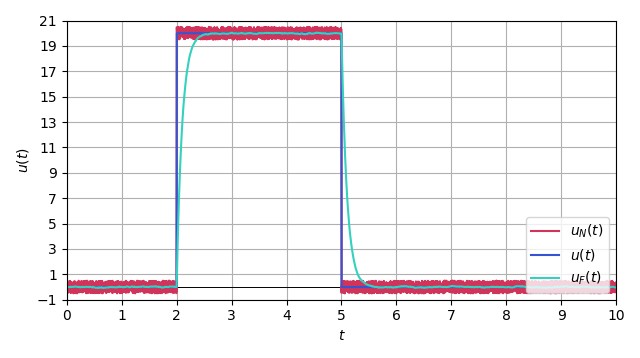
\includegraphics[width=0.66\textwidth]{sources/second/part1/a=20 T=0.1/1_signal_cmp.png}
    \caption{Графики исходного, зашумлённого и отфильтрованного сигналов при $a = 20$}
\end{figure}\vspace{-1em}
\begin{figure}[H]
    \begin{minipage}{0.49\textwidth}
        \centering 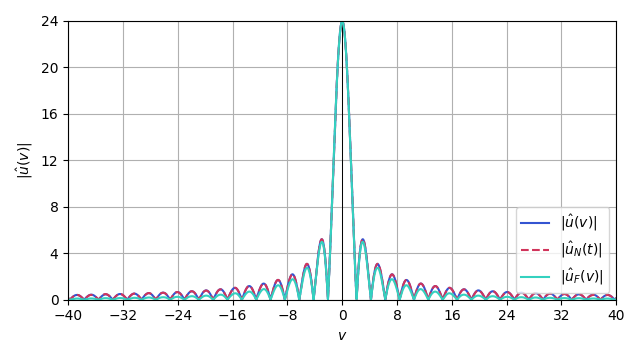
\includegraphics[width=\textwidth]{sources/second/part1/a=20 T=0.1/2_fft_cmp.png}
        \caption{Модули Фурье-образов сигналов при $a = 20$}
    \end{minipage}\hfill
    \begin{minipage}{0.49\textwidth}
        \centering \includegraphics[width=\textwidth]{sources/second/part1/a=20 T=0.1/3_filter.png}
        \caption{АЧХ фильтра при $a = 20$}
    \end{minipage}
\end{figure}
Как мы видим, увеличение амплитуды прямоугольной волны не изменило сглаживание на фронте и спаде, но уменьшило долю шума в отфильтрованном сигнале, потому как отношение амплитуды шума к общей амплитуде прямоугольной волны также уменьшилось. АЧХ фильтра не изменилась, потому как и постоянная времени не изменилась.\\[0.5em]
\textbf{Вывод:} фильтр первого порядка позволяет уменьшить шум в сигнале, но при этом сглаживает и сам сигнал. Постоянная времени фильтра $T$ влияет на степень сглаживания --- чем больше $T$, тем сильнее сглаживание, а амплитуды прямоугольной волны (параметр $a$) и шума (параметр $b$) влияют на долю шума в отфильтрованном сигнале.
\addsubsection{Специальный фильтр}
Теперь рассмотрим линейный фильтр второго порядка, передаточная функция которого выглядит так:
$$W_2(p) = \frac{\left( T_1p + 1 \right)^2}{\left( T_2p + 1 \right)\left( T_3p + 1 \right)} = \frac{T_1^2p^2+2T_1p+1}{T_2T_3p^2+\left( T_2+T_3 \right)p + 1}$$
Для выполнения задания понадобится сигнал только с гармоническим шумом, поэтому $b = 0$. Необходимо пропустить такой сигнал $u$ через фильтр, подобрать $T_1, T_2, T_3$ к различным значениям $d$ так, чтобы фильтр хорошо фильтровал шум и не сильно искажал сигнал, и исследовать как параметр $c$ влияет на фильтрацию.\\[0.5em]
Мы будем подбирать постоянные времени фильтра следующим образом:
\begin{itemize}
    \item Параметр $T_1$, находясь в числителе передаточной функции, влияет на усиление высоких частот. Так как это нам не требуется, положим $T_1 = 10^{-8}$ --- настолько минимальным, насколько это возможно.
    \item Беря во внимание, что для фильтра первого порядка действует правило частоты среза $\omega_c = \nicefrac{1}{T}$, подберём $T_2$ и $T_3$ так, чтобы они были связаны с частотой гармонического шума $d$.
\end{itemize}
Пусть $a = 5$ --- амплитуда прямоугольной волны, $c = 0.5$ --- амплитуда гармонического шума, $d = 18$ --- частота гармонического шума. Подберём постоянные времени фильтра так, чтобы он хорошо убирал гармонический шум (удвоение постоянных связано с тем, что их две в знаменателе):
$$T_1 = 10^{-8}\qquad T_2 = T_3 = \frac{2}{d} = \frac{1}{9}$$
Теперь посмотрим на сравнительные графики сигналов и модулей их Фурье-образов, а также на график АЧХ:
\begin{figure}[H]
    \centering 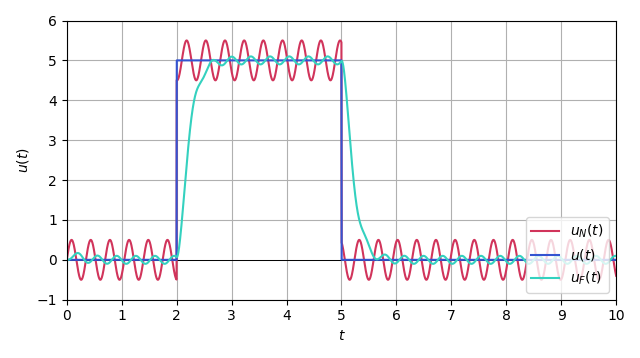
\includegraphics[width=0.66\textwidth]{sources/second/part2/c=0.5_d=18 T1=1e-08_T2=0.111_T3=0.111/1_signal_cmp.png}
    \caption{Графики исходного, зашумлённого и отфильтрованного сигналов при $c = 0.5$ и $d = 18$}
\end{figure}\vspace{-1em}
\begin{figure}[H]
    \begin{minipage}{0.49\textwidth}
        \centering 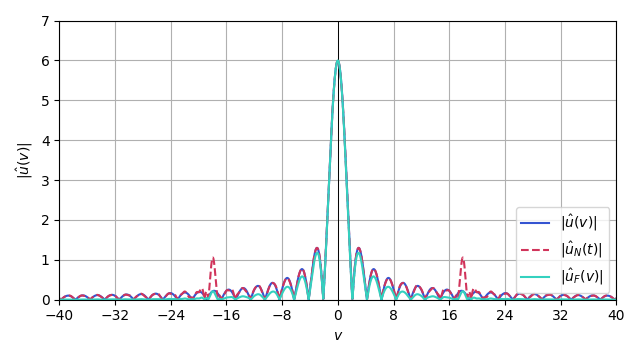
\includegraphics[width=\textwidth]{sources/second/part2/c=0.5_d=18 T1=1e-08_T2=0.111_T3=0.111/2_fft_cmp.png}
        \caption{Модули Фурье-образов при $c = 0.5$ и $d = 18$}
    \end{minipage}\hfill
    \begin{minipage}{0.49\textwidth}
        \centering \includegraphics[width=\textwidth]{sources/second/part2/c=0.5_d=18 T1=1e-08_T2=0.111_T3=0.111/3_filter.png}
        \caption{АЧХ фильтра при $c = 0.5$ и $d = 18$}
    \end{minipage}
\end{figure}
Мы можем наблюдать, что фильтр второго порядка хорошо убирает гармонический шум и при этом фронт и спад не сильно сглажены. На графике модулей Фурье-образов хорошо видно, что частота синусоидального шума заглушена. Если задать $T_2$ и $T_3$ ещё больше, то шум заглушится сильнее, но и в свою очередь фронт и спад прямоугольной волны будут также сглажены ещё сильнее.\newpage
Теперь рассмотрим шум с той же амплитудой, но с другой частотой, $d = 30$:
\begin{figure}[H]
    \centering 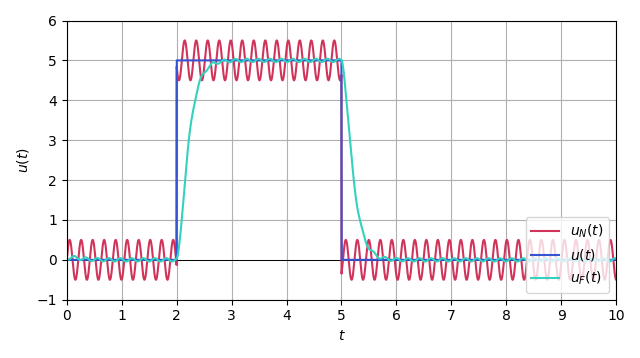
\includegraphics[width=0.66\textwidth]{sources/second/part2/c=0.5_d=30 T1=1e-08_T2=0.111_T3=0.111/1_signal_cmp.png}
    \caption{Графики исходного, зашумлённого и отфильтрованного сигналов при $c = 0.5$ и $d = 30$}
\end{figure}\vspace{-1em}
\begin{figure}[H]
    \begin{minipage}{0.49\textwidth}
        \centering 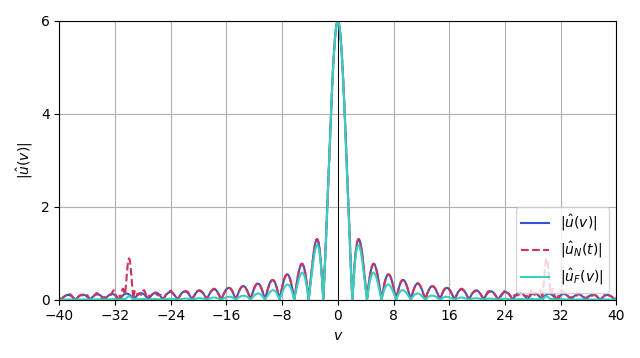
\includegraphics[width=\textwidth]{sources/second/part2/c=0.5_d=30 T1=1e-08_T2=0.111_T3=0.111/2_fft_cmp.png}
        \caption{Модули Фурье-образов при $c = 0.5$ и $d = 30$}
    \end{minipage}\hfill
    \begin{minipage}{0.49\textwidth}
        \centering \includegraphics[width=\textwidth]{sources/second/part2/c=0.5_d=30 T1=1e-08_T2=0.111_T3=0.111/3_filter.png}
        \caption{АЧХ фильтра при $c = 0.5$ и $d = 30$}
    \end{minipage}
\end{figure}
По АЧХ фильтра видно, что фильтр не изменился. На графике модулей Фурье-образов видно, что частота гармонического шума $d = 30$ также заглушена --- т.к. она находится ещё дальше от нулевой частоты, то гармонический шум заглушается ещё сильнее. Именно это мы наблюдаем на сравнительном графике сигналов --- амплитуда шума в отфильтрованном сигнале меньше. \newpage
Теперь попробуем увеличить амплитуду гармонического шума до $c = 3$, параметр $d$ оставим прежним:
\begin{figure}[H]
    \centering 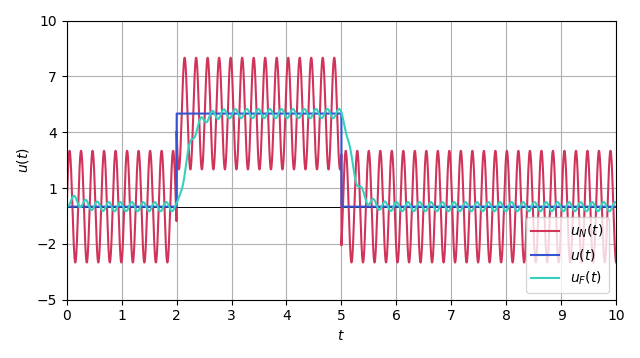
\includegraphics[width=0.66\textwidth]{sources/second/part2/c=3_d=30 T1=1e-08_T2=0.111_T3=0.111/1_signal_cmp.png}
    \caption{Графики исходного, зашумлённого и отфильтрованного сигналов при $c = 3$ и $d = 30$}
\end{figure}\vspace{-1em}
\begin{figure}[H]
    \begin{minipage}{0.49\textwidth}
        \centering 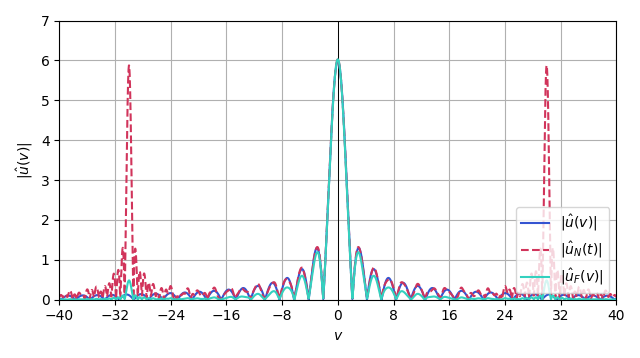
\includegraphics[width=\textwidth]{sources/second/part2/c=3_d=30 T1=1e-08_T2=0.111_T3=0.111/2_fft_cmp.png}
        \caption{Модули Фурье-образов при $c = 3$ и $d = 30$}
    \end{minipage}\hfill
    \begin{minipage}{0.49\textwidth}
        \centering \includegraphics[width=\textwidth]{sources/second/part2/c=3_d=30 T1=1e-08_T2=0.111_T3=0.111/3_filter.png}
        \caption{АЧХ фильтра при $c = 3$ и $d = 30$}
    \end{minipage}
\end{figure}
Как мы видим, увеличение амплитуды гармонического шума привело к увеличению амплитуды этого шума в отфильтрованном сигнале. На графике модулей Фурье-образов видно, что частота гармонического шума $d = 30$ выросла по амплитуде и при фильтрации заглушилась слабее, в сравнении с предыдущим примером.\\[0.5em]
\textbf{Вывод:} фильтр второго порядка позволяет убрать гармонический шум из сигнала, не сильно сглаживая сам сигнал. Постоянные времени фильтра $T_1,\ T_2,\ T_3$ влияют на степень фильтрации. Амплитуда гармонического шума $c$ влияет на долю шума в отфильтрованном сигнале --- чем больше $c$, тем больше шума в отфильтрованном сигнале.
\addsection{Сглаживание биржевых данных}
Теперь рассмотрим, как можно примененить линейные фильтры на практике. К примеру, рассмотрим скользящее среднее --- функция сглаживания данных, которая как раз основана на линейном фильтре первого порядка, который сглаживает шумы в графике котировок акции.\\[0.5em]
Реализуем скользящее среднее со следующими окнами: 1 день, 1 неделя, 1 месяц, 3 месяца, 1 год. Возьмём данные о котировках акции \verb|VKCO|, принадлежащих компании VK, за период с 02.07.20 (появление тикета на Мосбирже) по 29.12.23 (последний день торгов 2023 года) с интервалом в 1 день. Таким образом постоянная времени $T = 1$ будет эквивалентна одному дню. \newpage
Посмотрим, как работает линейный фильтр первого порядка для всех $T$:
\begin{figure}[H]
    \centering 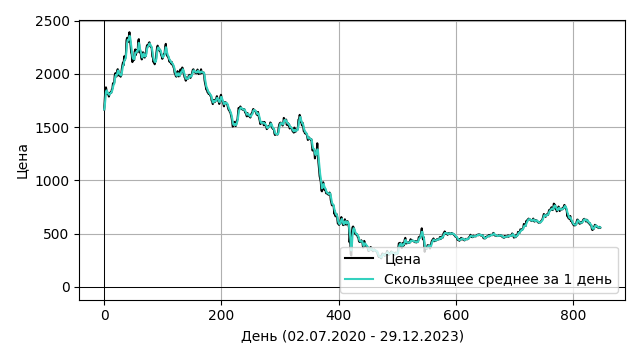
\includegraphics[width=0.66\textwidth]{sources/third/moving_average_1.png}
    \caption{График цены акции VKCO и скользящее среднее с окном в 1 день ($T = 1$)}
\end{figure}\vspace{-1em}
\begin{figure}[H]
    \centering 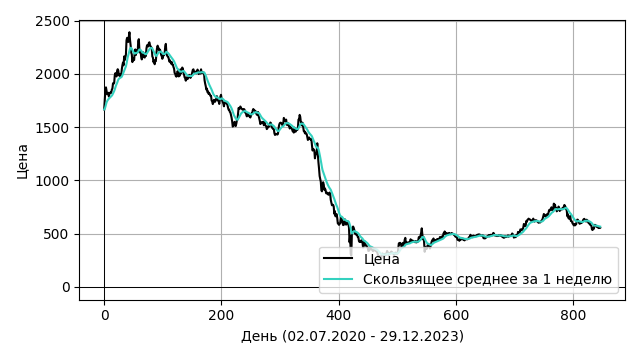
\includegraphics[width=0.66\textwidth]{sources/third/moving_average_7.png}
    \caption{График цены акции VKCO и скользящее среднее с окном в 1 неделю ($T = 7$)}
\end{figure}\vspace{-1em}
\begin{figure}[H]
    \centering 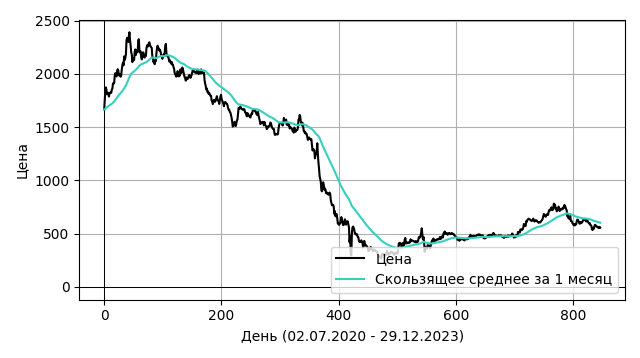
\includegraphics[width=0.66\textwidth]{sources/third/moving_average_30.png}
    \caption{График цены акции VKCO и скользящее среднее с окном в 1 месяц ($T = 30$)}
\end{figure}\vspace{-1em}
\begin{figure}[H]
    \centering 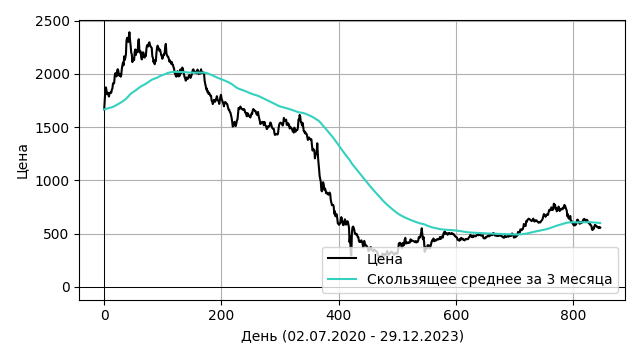
\includegraphics[width=0.66\textwidth]{sources/third/moving_average_90.png}
    \caption{График цены акции VKCO и скользящее среднее с окном в 3 месяца ($T = 90$)}
\end{figure}\vspace{-1em}
\begin{figure}[H]
    \centering 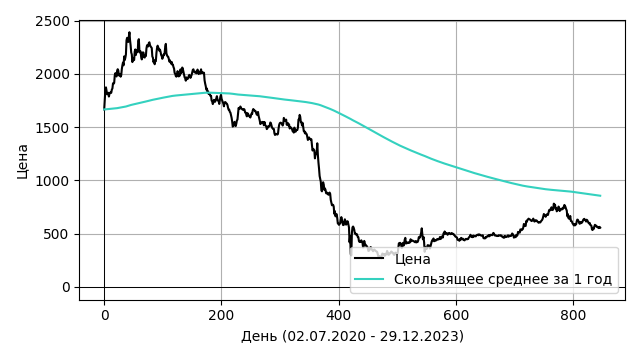
\includegraphics[width=0.66\textwidth]{sources/third/moving_average_365.png}
    \caption{График цены акции VKCO и скользящее среднее с окном в 1 год ($T = 365$)}
\end{figure}
\NB: при использовании \verb|lsim| в Python фильтрованный сигнал тоже начинается из нуля. Для этого необходимо добавить параметр \verb|X0=prices[0] * T|. После этого фильтрованный сигнал будет начинаться из той же точки, что и график цен.\\[0.5em]
\textbf{Вывод:} у линейных фильтров есть практическое применение --- не только фильтрация шумов в сигнале, но и сглаживание биржевых и в принципе любых других данных.
\end{document}